\documentclass[a4paper,12pt]{article}
\usepackage[utf8]{inputenc}
\usepackage[T1]{fontenc}
\usepackage[french]{babel}
\usepackage{geometry}
\usepackage{amsmath}
\usepackage{amssymb}
\usepackage{array}
\usepackage{graphicx}
\usepackage{booktabs}
\usepackage{float}
\usepackage{pgfplots}
\pgfplotsset{compat=1.18}

% Adjust margins to fit tables
\geometry{hmargin=2cm, vmargin=2cm}

\title{\textbf{Compte Rendu : Pendule Pesant Réversible}}
\author{Ilyas Tanam \\ Noha Maghfaoui}
\date{}

\begin{document}

\begin{titlepage}
    \centering
    \vspace*{2cm}
    
    {\Huge\bfseries Compte rendu Tp N°2\par}
    \vspace{1cm}
    {\LARGE Pendule Réversible\par}
    \vspace{2cm}
    
    % Add your image here
    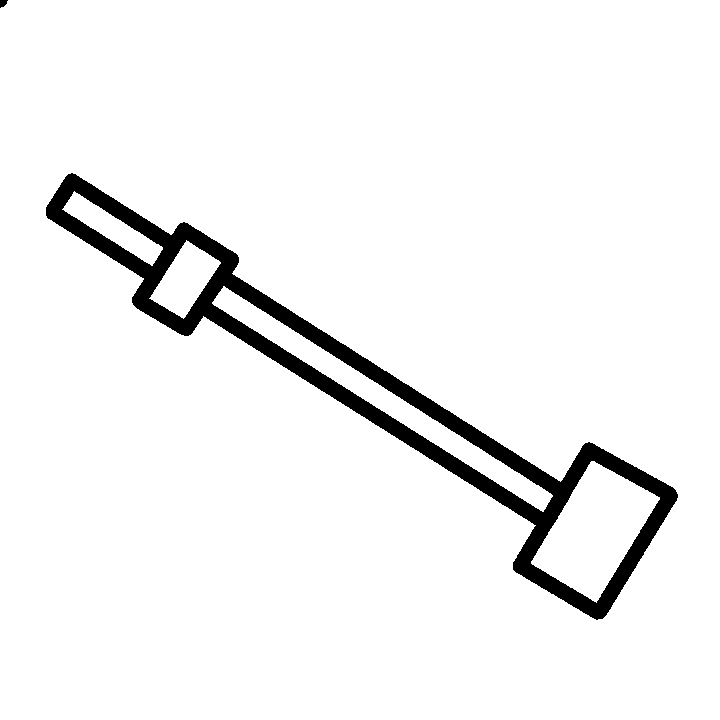
\includegraphics[width=0.4\textwidth]{pnd.png}
    % Replace "your-image-filename.png" with your actual image file
    
    \vspace{2cm}
    
    {\Large réalisé par:\par}
    \vspace{0.5cm}
    {\large Ilyas Zanan \hspace{2cm} Noha Maghfoul\par}
    
    \vspace{1.5cm}
    
    {\Large encadré par:\par}
    \vspace{0.5cm}
    {\large Pr. Mohamed AHD\par}
    
    \vspace{1.5cm}
    
    {\Large responsable:\par}
    \vspace{0.5cm}
    {\large Pr. Mohamed GOUIGHRI\par}
    
    \vfill
    
\end{titlepage}

\newpage

\begin{center}
    \textbf{\large Compte rendu Pendule pesant reversible}
\end{center}

\section{Isochronisme des petites oscillations}
\begin{enumerate}
    \item Tableau des mesures  
\begin{table}[H]
    \centering
    \renewcommand{\arraystretch}{1.5}
    \begin{tabular}{|c|c|c|c|c|c|c|c|c|c|}
    \hline
    temps(s) & $t_1$ & $t_2$ & $t_3$ & $t_m$ & $\Delta t_m$ & $\Delta t_{ch}$ & $\Delta t$ & $T(s)$ & $\Delta T(s)$ \\
    \hline
    $\theta_1$ & 16,72 & 16,12 & 16,30 & 16,38 & 0,34 & 0,1 & 0,44 & 1,638 & 0,03 \\
    \hline
    $\theta_2$ & 15,55 & 16,21 & 16,19 & 15,98 & 0,43 & 0,1 & 0,53 & 1,598 & 0,04 \\
    \hline
    \end{tabular}
\end{table}

    \item
En comparant les 2 valeurs de $T$ pour $\theta_1$ et $\theta_2$, on en déduit que la période ne dépend pas de l'angle $\theta$ (il y a une différence négligeable entre les valeurs due à la précision temps au cours de l'expérience).


\end{enumerate}
\section{Détermination expérimentales des axes réciproques du pendule réversible}

\begin{enumerate}
    \item Tableau des mesures 
\begin{table}[H]
    \centering
    \renewcommand{\arraystretch}{1.4}
    \begin{tabular}{|c|c|c|c|c|c|c|c|}
    \hline
    $x (\text{cm})$ & $\Delta x$ & \multicolumn{2}{c|}{$t = 10T (s)$} & $\Delta t (s)$ & $T = t/10 (s)$ & $\Delta T$ & $t_m$ \\
    \hline
    10 & 0,1 & 17,93 & 17,90 & 0,13 & 1,79 & 0,013 & 17,915 \\
    \hline
    20 & 0,1 & 16,35 & 16,43 & 0,18 & 1,639 & 0,018 & 16,39 \\
    \hline
    30 & 0,1 & 16,27 & 16,10 & 0,27 & 1,618 & 0,027 & 16,185 \\
    \hline
    40 & 0,1 & 15,60 & 15,56 & 0,14 & 1,558 & 0,014 & 15,58 \\
    \hline
    50 & 0,1 & 15,73 & 15,78 & 0,15 & 1,575 & 0,015 & 15,755 \\
    \hline
    60 & 0,1 & 16,73 & 17,41 & 0,78 & 1,707 & 0,078 & 17,07 \\
    \hline
    70 & 0,1 & 28,66 & 28,98 & 0,42 & 2,882 & 0,042 & 28,82 \\
    \hline
    80 & 0,1 & 27,42 & 26,38 & 1,22 & 2,609 & 0,122 & 26,09 \\
    \hline
    90 & 0,1 & 17,35 & 17,3 & 0,15 & 1,732 & 0,015 & 17,325 \\
    \hline
    96 & 0,1 & 15,93 & 15,85 & 0,18 & 1,589 & 0,018 & 15,89 \\
    \hline
    \end{tabular}
\end{table}

\noindent \textbf{Remarque :} Les relations utilisées étaient données en TP, à savoir :
\[ \Delta t_m = \sup|t_m - t_i| \quad , \quad T = \frac{t_m}{10} \quad , \quad \Delta T = \frac{\Delta t}{10} \quad , \quad \Delta t = \Delta t_m + \Delta t_{ch} \]

    \item Graphe de T en fct de x

\begin{center}
    \begin{tikzpicture}
        \begin{axis}[
                width=0.9\textwidth,  % Makes it 90% of text width
                height=0.6\textwidth, % Adjust height proportionally
                title={Graphe de la période $T$ en fonction de $x$},
                xlabel={$x$ (cm)},
                ylabel={$T$ (s)},
                xmin=0, xmax=100,
                ymin=1.4, ymax=3,
                grid=both,
                minor tick num=1,
                axis lines=left,
                legend pos=north east,
                /pgf/number format/.cd,
                use comma,
                1000 sep={},
                % Add T1 and T2 as extra y-axis ticks
                ytick={1.5, 2, 2.5, 3},
                extra y ticks={1.65, 1.70},
                extra y tick labels={$T_1$, $T_2$},
                extra y tick style={
                    tick label style={anchor=east, xshift=3pt,font=\tiny},
                    grid=none
                }
            ]
    
        % --- The Vertical Asymptote at x=80 ---
        \draw [red, dashed, thick] (axis cs:80, \pgfkeysvalueof{/pgfplots/ymin}) -- (axis cs:80, \pgfkeysvalueof{/pgfplots/ymax});
    
        % --- Horizontal Lines for T1 and T2 ---
        % Note: T is on the y-axis, so specific T values form horizontal lines
        
        % Line for T2 = 1.70
        \addplot [domain=0:100, samples=2, dashed, teal, thick] {1.70};
    
        % Line for T1 = 1.65
        \addplot [domain=0:100, samples=2, dashed, orange, thick] {1.65};
    
        % --- The Curve (Left of Asymptote x < 80) ---
        % I combined table data with the specific intersection points to make it accurate
        \addplot [
            blue,
            thick,
            smooth,
            tension=0.6
        ] coordinates {
            (10, 1.79)
            (20, 1.639)
            (30, 1.618)
            (40, 1.558)
            (50, 1.575)
            (60, 1.707)
            (70, 2.882)
            (76, 5.0) % Artificial point to force asymptote direction
        };
    
        % --- The Curve (Right of Asymptote x > 80) ---
        \addplot [
            blue,
            thick,
            smooth,
            tension=0.6
        ] coordinates {
            (87.95, 5.0) % Artificial point to force asymptote direction
            (88.7, 4.5)
            (89, 2.5)
            (89.5, 2)
            (90, 1.732) 
            (96, 1.589)
        };
    
        % --- Plotting the Intersection Points (Visual Markers) ---
        
        % Points for T = 1.65 (O1, O2, O3)
        \addplot[
            only marks,
            mark=*,
            color=orange,
            mark size=2pt
        ] coordinates {
            (18.5, 1.65)
            (58.5, 1.65)
            (92.5, 1.65)
        };
        
        % Points for T = 1.70 (O'1, O'2, O'3)
        \addplot[
            only marks,
            mark=*,
            color=teal,
            mark size=2pt
        ] coordinates {
            (15.0, 1.70)
            (59.5, 1.70)
            (91.0, 1.70)
        };
    
        % Labels for the points
        \node[below left, font=\footnotesize] at (axis cs:18.5, 1.65) {$O_1$};
        \node[below right, font=\footnotesize] at (axis cs:57.0, 1.65) {$O_2$};
        \node[below left, font=\footnotesize] at (axis cs:92.5, 1.65) {$O_3$};
    
        \node[above left, font=\footnotesize] at (axis cs:18.0, 1.70) {$O'_1$};
        \node[above right, font=\footnotesize] at (axis cs:59.5, 1.70) {$O'_2$};
        \node[above right, font=\footnotesize] at (axis cs:91.0, 1.70) {$O'_3$};
    
        \end{axis}
    \end{tikzpicture}
\end{center}

    \item Les axes horizontaux les deux axes sont présentés dans le graph

    \item Coordonnées des points 
On relève : $T_1 = 1,65 \, s$ et $T_2 = 1,70 \, s$. \\
Les coordonnées des points sont :
\begin{align*}
O_1 &: (18,5 \ ; \ 1,65) & O'_1 &: (18,0 \ ; \ 1,70) \\
O_2 &: (57,0 \ ; \ 1,65) & O'_2 &: (59,5 \ ; \ 1,70) \\
O_3 &: (92,5 \ ; \ 1,65) & O'_3 &: (91,0 \ ; \ 1,70)
\end{align*}

    \item Calcul des longueurs 
\begin{align*}
L &= X_3 - X_1 & L' &= X'_3 - X'_1 \\
L &= 92,5 - 18,5 & L' &= 91,0 - 18,0 \\
\mathbf{L} &= \mathbf{74 \, cm} & \mathbf{L'} &= \mathbf{73 \, cm}
\end{align*}

    \item Calcul de l'accélération de la pesanteur g 

On sait que :
\[ T = 2\pi \sqrt{\frac{L}{g}} \]
Donc :
\[ g = 4\pi^2 \frac{L}{T^2} \]

\noindent \textbf{Application Numérique :}

Pour $g_1$ (avec $L=74\text{cm}$ et $T=1,65\text{s}$) :
\[ g_1 = 4\pi^2 \times \frac{74 \times 10^{-2}}{(1,65)^2} \implies \boxed{g_1 \approx 10,73 \, m/s^2} \]

Pour $g_2$ (avec $L'=73\text{cm}$ et $T=1,70\text{s}$) :
\[ g_2 = 4\pi^2 \times \frac{73 \times 10^{-2}}{(1,70)^2} \implies \boxed{g_2 \approx 9,968 \, m/s^2} \]

\noindent \textbf{Moyenne :}
\[ g_m = \frac{g_1 + g_2}{2} = \frac{10,73 + 9,968}{2} \implies \boxed{g_m = 10,35 \, m/s^2} \]

\noindent \textbf{Incertitude :}
\[ \Delta g_m = \frac{|g_1 - g_2|}{2} = \frac{|10,73 - 9,968|}{2} \implies \boxed{\Delta g_m = 0,39 \, m/s^2} \]

\noindent \textbf{Résultat final :}
\begin{center}
    \framebox[1.1\width]{$g = (10,35 \pm 0,39) \, m/s^2$}
\end{center}

    \item conclusion et comparaison
La valeur théorique est de $g_{th} = 9,81 \, m/s^2$.
La valeur expérimentale est de $10,35 \, m/s^2$, elle est légèrement supérieure à la théorique.

\noindent \textbf{L'erreur relative est :}
\[ \varepsilon = \frac{|10,35 - 9,81|}{9,81} \approx 5,5\% \]

La méthode du pendule réversible a permis de déterminer l'ordre de grandeur de $g$. L'écart de 5,5\% s'explique par :
\begin{itemize}
    \item Le temps de la réaction humaine.
    \item Les frottements au niveau de l'axe de rotation.
\end{itemize}

\end{enumerate}

\end{document}